\documentclass[tikz,border=3.14mm]{standalone}
\usepackage{tikz}
\usepackage{pgfplots}
\usepackage{xcolor}
\usepackage{amsmath}
\usetikzlibrary{shapes,arrows,positioning,calc,decorations.pathreplacing,backgrounds}
\pgfplotsset{compat=1.17}

% Define colors
\definecolor{quantum}{RGB}{0,150,255}
\definecolor{ai}{RGB}{50,205,50}
\definecolor{blockchain}{RGB}{255,140,0}
\definecolor{human}{RGB}{255,69,0}
\definecolor{background}{RGB}{248,249,250}

\begin{document}

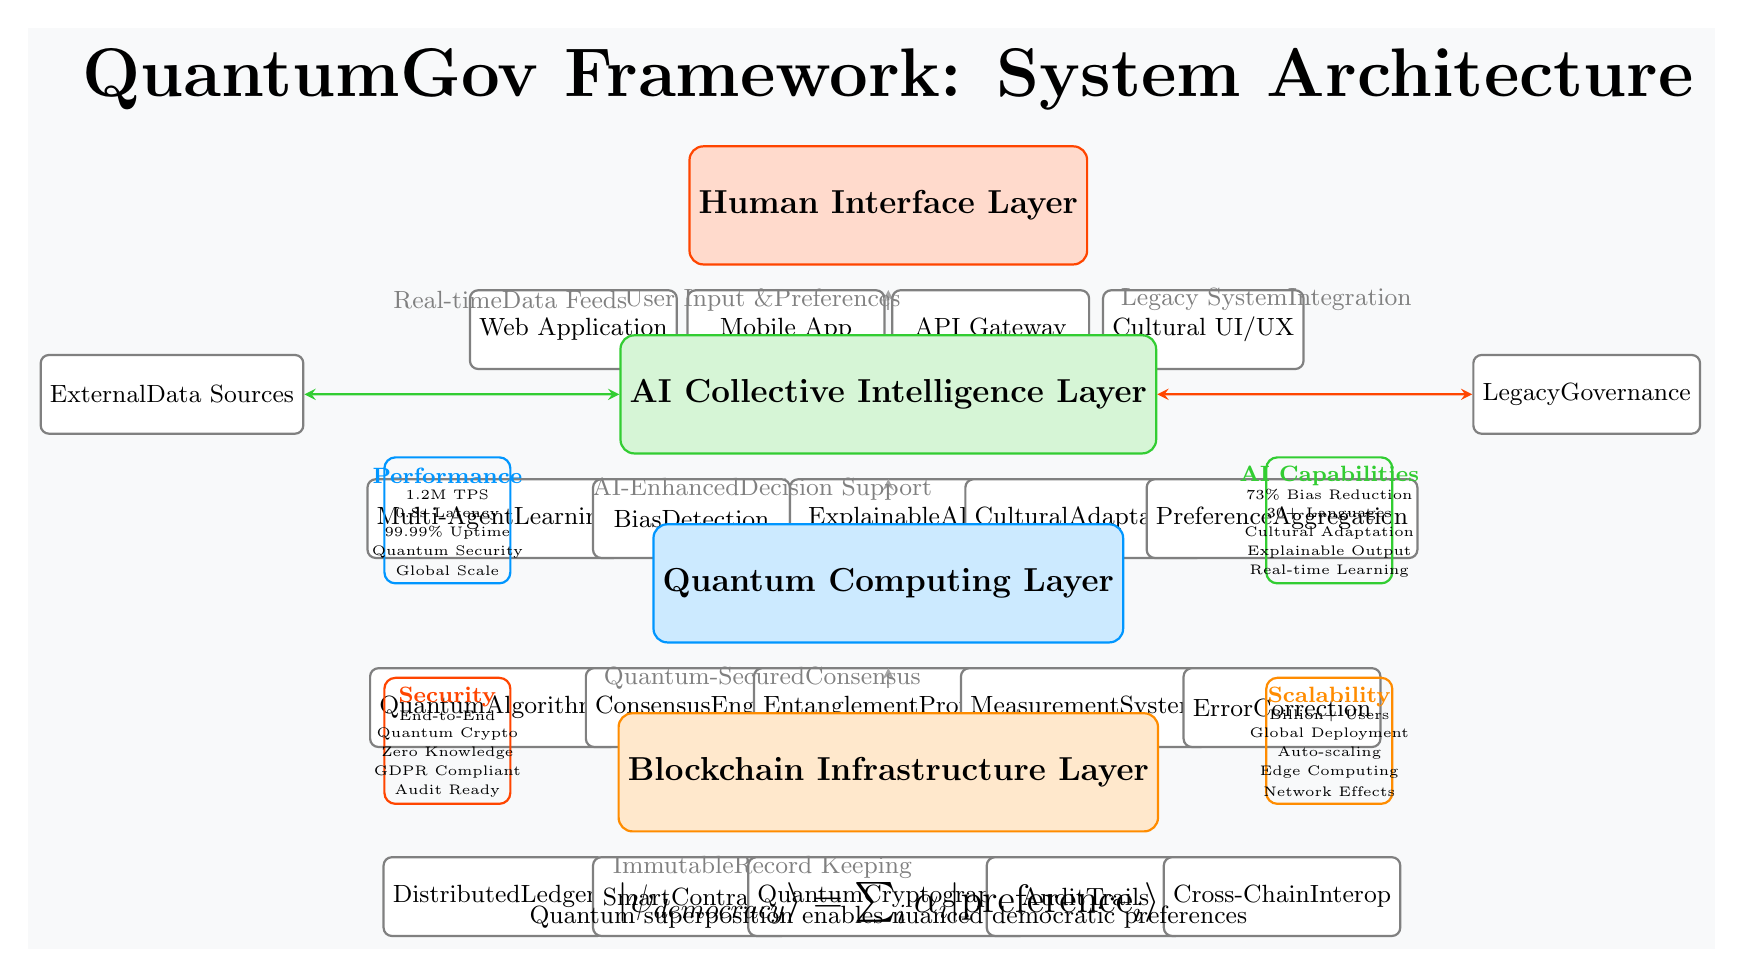
\begin{tikzpicture}[
    scale=0.8,
    node distance=1.5cm,
    thick,
    >=stealth,
    background rectangle/.style={fill=background},
    show background rectangle,
    quantum_box/.style={
        rectangle,
        draw=quantum,
        fill=quantum!20,
        minimum width=3cm,
        minimum height=1.5cm,
        rounded corners=5pt,
        text centered,
        font=\large\bfseries
    },
    ai_box/.style={
        rectangle,
        draw=ai,
        fill=ai!20,
        minimum width=3cm,
        minimum height=1.5cm,
        rounded corners=5pt,
        text centered,
        font=\large\bfseries
    },
    blockchain_box/.style={
        rectangle,
        draw=blockchain,
        fill=blockchain!20,
        minimum width=3cm,
        minimum height=1.5cm,
        rounded corners=5pt,
        text centered,
        font=\large\bfseries
    },
    human_box/.style={
        rectangle,
        draw=human,
        fill=human!20,
        minimum width=3cm,
        minimum height=1.5cm,
        rounded corners=5pt,
        text centered,
        font=\large\bfseries
    },
    component/.style={
        rectangle,
        draw=gray,
        fill=white,
        minimum width=2.5cm,
        minimum height=1cm,
        rounded corners=3pt,
        text centered,
        font=\small
    },
    arrow/.style={
        ->,
        thick,
        color=gray!70
    }
]

% Title
\node[font=\Huge\bfseries] at (0,12) {QuantumGov Framework: System Architecture};

% Layer 4: Human Interface Layer
\node[human_box] (human_interface) at (0,10) {Human Interface Layer};
\node[component, below=0.3cm of human_interface, xshift=-4cm] (web_app) {Web Application};
\node[component, below=0.3cm of human_interface, xshift=-1.3cm] (mobile_app) {Mobile App};
\node[component, below=0.3cm of human_interface, xshift=1.3cm] (api_gateway) {API Gateway};
\node[component, below=0.3cm of human_interface, xshift=4cm] (ui_framework) {Cultural UI/UX};

% Layer 3: AI Collective Intelligence Layer
\node[ai_box] (ai_layer) at (0,7) {AI Collective Intelligence Layer};
\node[component, below=0.3cm of ai_layer, xshift=-5cm] (multi_agent) {Multi-Agent\\Learning};
\node[component, below=0.3cm of ai_layer, xshift=-2.5cm] (bias_detection) {Bias\\Detection};
\node[component, below=0.3cm of ai_layer, xshift=0cm] (explainable_ai) {Explainable\\AI};
\node[component, below=0.3cm of ai_layer, xshift=2.5cm] (cultural_adapt) {Cultural\\Adaptation};
\node[component, below=0.3cm of ai_layer, xshift=5cm] (preference_agg) {Preference\\Aggregation};

% Layer 2: Quantum Computing Layer
\node[quantum_box] (quantum_layer) at (0,4) {Quantum Computing Layer};
\node[component, below=0.3cm of quantum_layer, xshift=-5cm] (quantum_algorithms) {Quantum\\Algorithms};
\node[component, below=0.3cm of quantum_layer, xshift=-2.5cm] (consensus_engine) {Consensus\\Engine};
\node[component, below=0.3cm of quantum_layer, xshift=0cm] (entanglement) {Entanglement\\Protocol};
\node[component, below=0.3cm of quantum_layer, xshift=2.5cm] (measurement) {Measurement\\System};
\node[component, below=0.3cm of quantum_layer, xshift=5cm] (error_correction) {Error\\Correction};

% Layer 1: Blockchain Infrastructure Layer
\node[blockchain_box] (blockchain_layer) at (0,1) {Blockchain Infrastructure Layer};
\node[component, below=0.3cm of blockchain_layer, xshift=-5cm] (distributed_ledger) {Distributed\\Ledger};
\node[component, below=0.3cm of blockchain_layer, xshift=-2.5cm] (smart_contracts) {Smart\\Contracts};
\node[component, below=0.3cm of blockchain_layer, xshift=0cm] (crypto_security) {Quantum\\Cryptography};
\node[component, below=0.3cm of blockchain_layer, xshift=2.5cm] (audit_trails) {Audit\\Trails};
\node[component, below=0.3cm of blockchain_layer, xshift=5cm] (interop) {Cross-Chain\\Interop};

% External Systems
\node[component, left=4cm of ai_layer] (external_data) {External\\Data Sources};
\node[component, right=4cm of ai_layer] (governance_systems) {Legacy\\Governance};

% Arrows between layers
\foreach \start/\end in {human_interface/ai_layer, ai_layer/quantum_layer, quantum_layer/blockchain_layer} {
    \draw[arrow] ([yshift=-0.7cm]\start.south) -- ([yshift=0.7cm]\end.north);
}

% Bidirectional arrows for external systems
\draw[<->, thick, color=ai] (external_data) -- (ai_layer);
\draw[<->, thick, color=human] (governance_systems) -- (ai_layer);

% Data flow annotations
\node[font=\small, color=gray] at (-6,8.5) {Real-time\\Data Feeds};
\node[font=\small, color=gray] at (6,8.5) {Legacy System\\Integration};
\node[font=\small, color=gray] at (-2,8.5) {User Input \&\\Preferences};
\node[font=\small, color=gray] at (-2,5.5) {AI-Enhanced\\Decision Support};
\node[font=\small, color=gray] at (-2,2.5) {Quantum-Secured\\Consensus};
\node[font=\small, color=gray] at (-2,-0.5) {Immutable\\Record Keeping};

% Performance metrics boxes
\draw[quantum, thick, rounded corners] (-8,6) rectangle (-6,4);
\node[font=\footnotesize\bfseries, color=quantum] at (-7,5.7) {Performance};
\node[font=\tiny] at (-7,5.4) {1.2M TPS};
\node[font=\tiny] at (-7,5.1) {0.8s Latency};
\node[font=\tiny] at (-7,4.8) {99.99\% Uptime};
\node[font=\tiny] at (-7,4.5) {Quantum Security};
\node[font=\tiny] at (-7,4.2) {Global Scale};

\draw[ai, thick, rounded corners] (6,6) rectangle (8,4);
\node[font=\footnotesize\bfseries, color=ai] at (7,5.7) {AI Capabilities};
\node[font=\tiny] at (7,5.4) {73\% Bias Reduction};
\node[font=\tiny] at (7,5.1) {30+ Languages};
\node[font=\tiny] at (7,4.8) {Cultural Adaptation};
\node[font=\tiny] at (7,4.5) {Explainable Output};
\node[font=\tiny] at (7,4.2) {Real-time Learning};

% Mathematical formulation
\node[font=\Large, below=0.5cm of blockchain_layer] {$|\psi_{democracy}\rangle = \sum_{i} \alpha_i |\text{preference}_i\rangle$};
\node[font=\small, below=0.8cm of blockchain_layer] {Quantum superposition enables nuanced democratic preferences};

% Security and compliance indicators
\draw[human, thick, rounded corners] (-8,2.5) rectangle (-6,0.5);
\node[font=\footnotesize\bfseries, color=human] at (-7,2.2) {Security};
\node[font=\tiny] at (-7,1.9) {End-to-End};
\node[font=\tiny] at (-7,1.6) {Quantum Crypto};
\node[font=\tiny] at (-7,1.3) {Zero Knowledge};
\node[font=\tiny] at (-7,1.0) {GDPR Compliant};
\node[font=\tiny] at (-7,0.7) {Audit Ready};

\draw[blockchain, thick, rounded corners] (6,2.5) rectangle (8,0.5);
\node[font=\footnotesize\bfseries, color=blockchain] at (7,2.2) {Scalability};
\node[font=\tiny] at (7,1.9) {Billion+ Users};
\node[font=\tiny] at (7,1.6) {Global Deployment};
\node[font=\tiny] at (7,1.3) {Auto-scaling};
\node[font=\tiny] at (7,1.0) {Edge Computing};
\node[font=\tiny] at (7,0.7) {Network Effects};

\end{tikzpicture}

\end{document}